\chapter{Recherche}
\label{sec:recherche}
Die Recherche nimmt sich dem Thema Data Mining an und erklärt die einzelnen Schritte, welche dabei ausgeführt werden. Danach werden die verschiedenen Gruppen von Algorithmen, die Disziplinen, vorgestellt. 

\section{Prozess des Data Mining}
\label{sec:recherche:dataminingtechniken}
Unter Data Mining versteht man die Anwendung von statistischen Methoden auf grossen Datenmengen mit dem Ziel, neue Erkenntnisse zu gewinnen.

Data Mining sieht folgende Schritte vor:
\begin{enumerate}
	\item Datenbeschaffung
	\item Daten vorbereiten
	\item Methoden zur Gewinnung von Informationen anwenden
	\item Überprüfung der Resultate
\end{enumerate}

Schritt 1 ist die Beschaffung der Daten, welche analysiert werden sollen (siehe \cref{sec:recherche:datenbeschaffung} \nameref{sec:recherche:datenbeschaffung}). 

Die Vorbereitung der Daten Bereinigt, Transformiert und Reduziert Informationen und wird im \cref{sec:recherche:datenvorbereitung} \nameref{sec:recherche:datenvorbereitung} beschrieben.

Der dritte Punkt ist das eigentliche Datengewinnung. Dabei werden Methoden des Data Mining auf die Daten angewendet. Mögliche Vorgehensweisen werden im \cref{sec:recherche:dataminingtechniken:disziplinen} \nameref{sec:recherche:dataminingtechniken:disziplinen} beschrieben.

Beim letzten Schritt werden die Resultate überprüft. Ist das Resultat nicht zufriedenstellend, so werden Punkt 2-4 wiederholt.

\section{Disziplinen im Data Mining}
\label{sec:recherche:dataminingtechniken:disziplinen}
Die Auswahl der Algorithmen ist riesig. Alle zu beschreiben würde eine Arbeit für sich selbst benötigen. Deshalb wurde die Auswahl der Techniken eingeschränkt auf die im Buch \cite{data_mining_concepts_and_techniques}. 
 
Vorgestellt werden fünf Techniken welche zum Teil ganz unterschiedliche Problemstellungen angehen. Cluster analysis und Classification unterteilen die Datenmenge in ähnliche Gruppen. Association rule learning, Lineare Regression und Collaborative Filtering versuchen anhand bestehender Daten werte für neue Datensätze vorherzusagen. Nachfolgend werden diese Techniken genauer erläutert.

\subsection{Association rule learning}
\label{sec:recherche:dataminingtechniken:disziplinen:association}
Bei Association rule learning (Assoziationsanalyse) handelt es sich um \gls{supervisedlearning} wobei Korrelationen zwischen Attributen aufgedeckt werden. Bei einer Warenkorbanalyse kann dadurch erkannt werden, welche Produkte die Kunden oft zusammen eingekaufen.

Der Prozess in der Assoziationsanalyse besteht aus zwei Schritten. Zuerst werden häufig auftretende Attributkombinationen gesucht, aus welchen anschliessend Regeln generiert werden\footcite{association_rule_learning_2017-01-05}.

Im Falle einer Warenkorbanalyse ein Beispiel einer Regel: "`Samstags wenn ein Kunde Käse und Brot kauft, dann kauft er auch Liquor"'. Oder im Falle von Interhome "Wenn ein Kunde eine Ferienwohnung mit Pool am Meer bucht, dann besitzt das Objekt auch eine Klimaanlage".

\subsection{Classification}
\label{sec:recherche:dataminingtechniken:disziplinen:classification}
Das Ziel der Classification (Klassifikation) ist es, eine Instanz einer Klasse zuzuweisen. Dies könnte die Kreditwürdigkeit eines Kunden sein. Die Klassen sind dabei vordefiniert, wodurch es um ein \gls{supervisedlearning} handelt.

Es gibt verschiedene Techniken für die Zuweisung einer Instanz zu einer Klasse. Es können Entscheidungsregeln, Bayes-Klassifikatoren, neuronale Netze und weitere verwendet werden\footcite{comparision_classification_algorithms}. Entscheidungsregeln können als Bäume dargestellt werden und sind visuell einfach verständlich.

\begin{figure}[H]
	\centering
	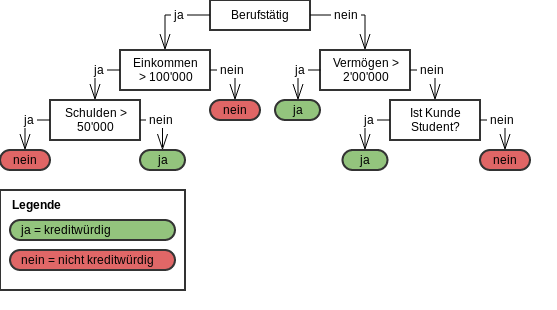
\includegraphics[width=0.8\textwidth]{images/decision_tree.png}
	\caption{Entscheidungsbaum für die Kreditwürdigkeit eines Kunden.}
	\label{fig:recherche:dataminingtechniken:disziplinen:classification}
\end{figure}

\cref{fig:recherche:dataminingtechniken:disziplinen:classification} zeigt einen Entscheidungsbaum, welcher von oben nach unten durchlaufen wird. Die Quadrate sind Entscheidungen, und bei den Ovalen handelt es sich um Zuweisungen zu der Klasse "`kreditwürdig"'.

% Evt. noch was schreiben über Training- und Testdaten

\subsection{Lineare Regression}
\label{sec:recherche:dataminingtechniken:disziplinen:regression}
Bei der linearen Regression wird ein Wert $Y$ prognostiziert welcher Abhängig von mehreren Variablen $X_p$ ist. Man spricht von einer abhängiger Variable $Y$, einer (oder mehrere) unabhängige Grösse(n) $X_p$ und einer (oder mehrere) unbekannte(n) Parameter $\beta_p$. Dabei werden bestehende Daten auf einem Koordinatensystem aufgetragen und eine Funktion gesucht, welche die Messungen möglichst genau annähert. Für gegebene unabhängige Variablen kann somit die abhängige Grösse errechnet werden.

Die \cref{eq:recherche:dataminingtechniken:disziplinen:regression:1} zeigt die Generalisierte Gleichung der linearen Regression.

\begin{equation} \label{eq:recherche:dataminingtechniken:disziplinen:regression:1}
Y = \beta_0 + \beta_1 * X_1 + \dots + \beta_p * X_p + \epsilon
\end{equation}
Benötigt wird ein Datensatz mit $Y$ und $X_p$ Paaren um die $\beta$ Parameter zu lernen (man spricht von einem Modell). Da die Messwerte oft nicht auf der Regressionslinie liegen, wird ein Fehleranteil $\epsilon$ benötigt\footcite{Einfache_lineare_Regression_2017-03-14}.

Bei der einfachen linearen Regression wird nur ein $X$ gegeben.

\begin{equation} \label{eq:recherche:dataminingtechniken:disziplinen:regression:2}
Y = \beta_0 + \beta_1 * X_1 + \epsilon
\end{equation}

\cref{fig:recherche:dataminingtechniken:disziplinen:regression} zeigt das Resultat einer einfachen linearen Regression.

\begin{figure}[H]
	\RawFloats
	\centering
	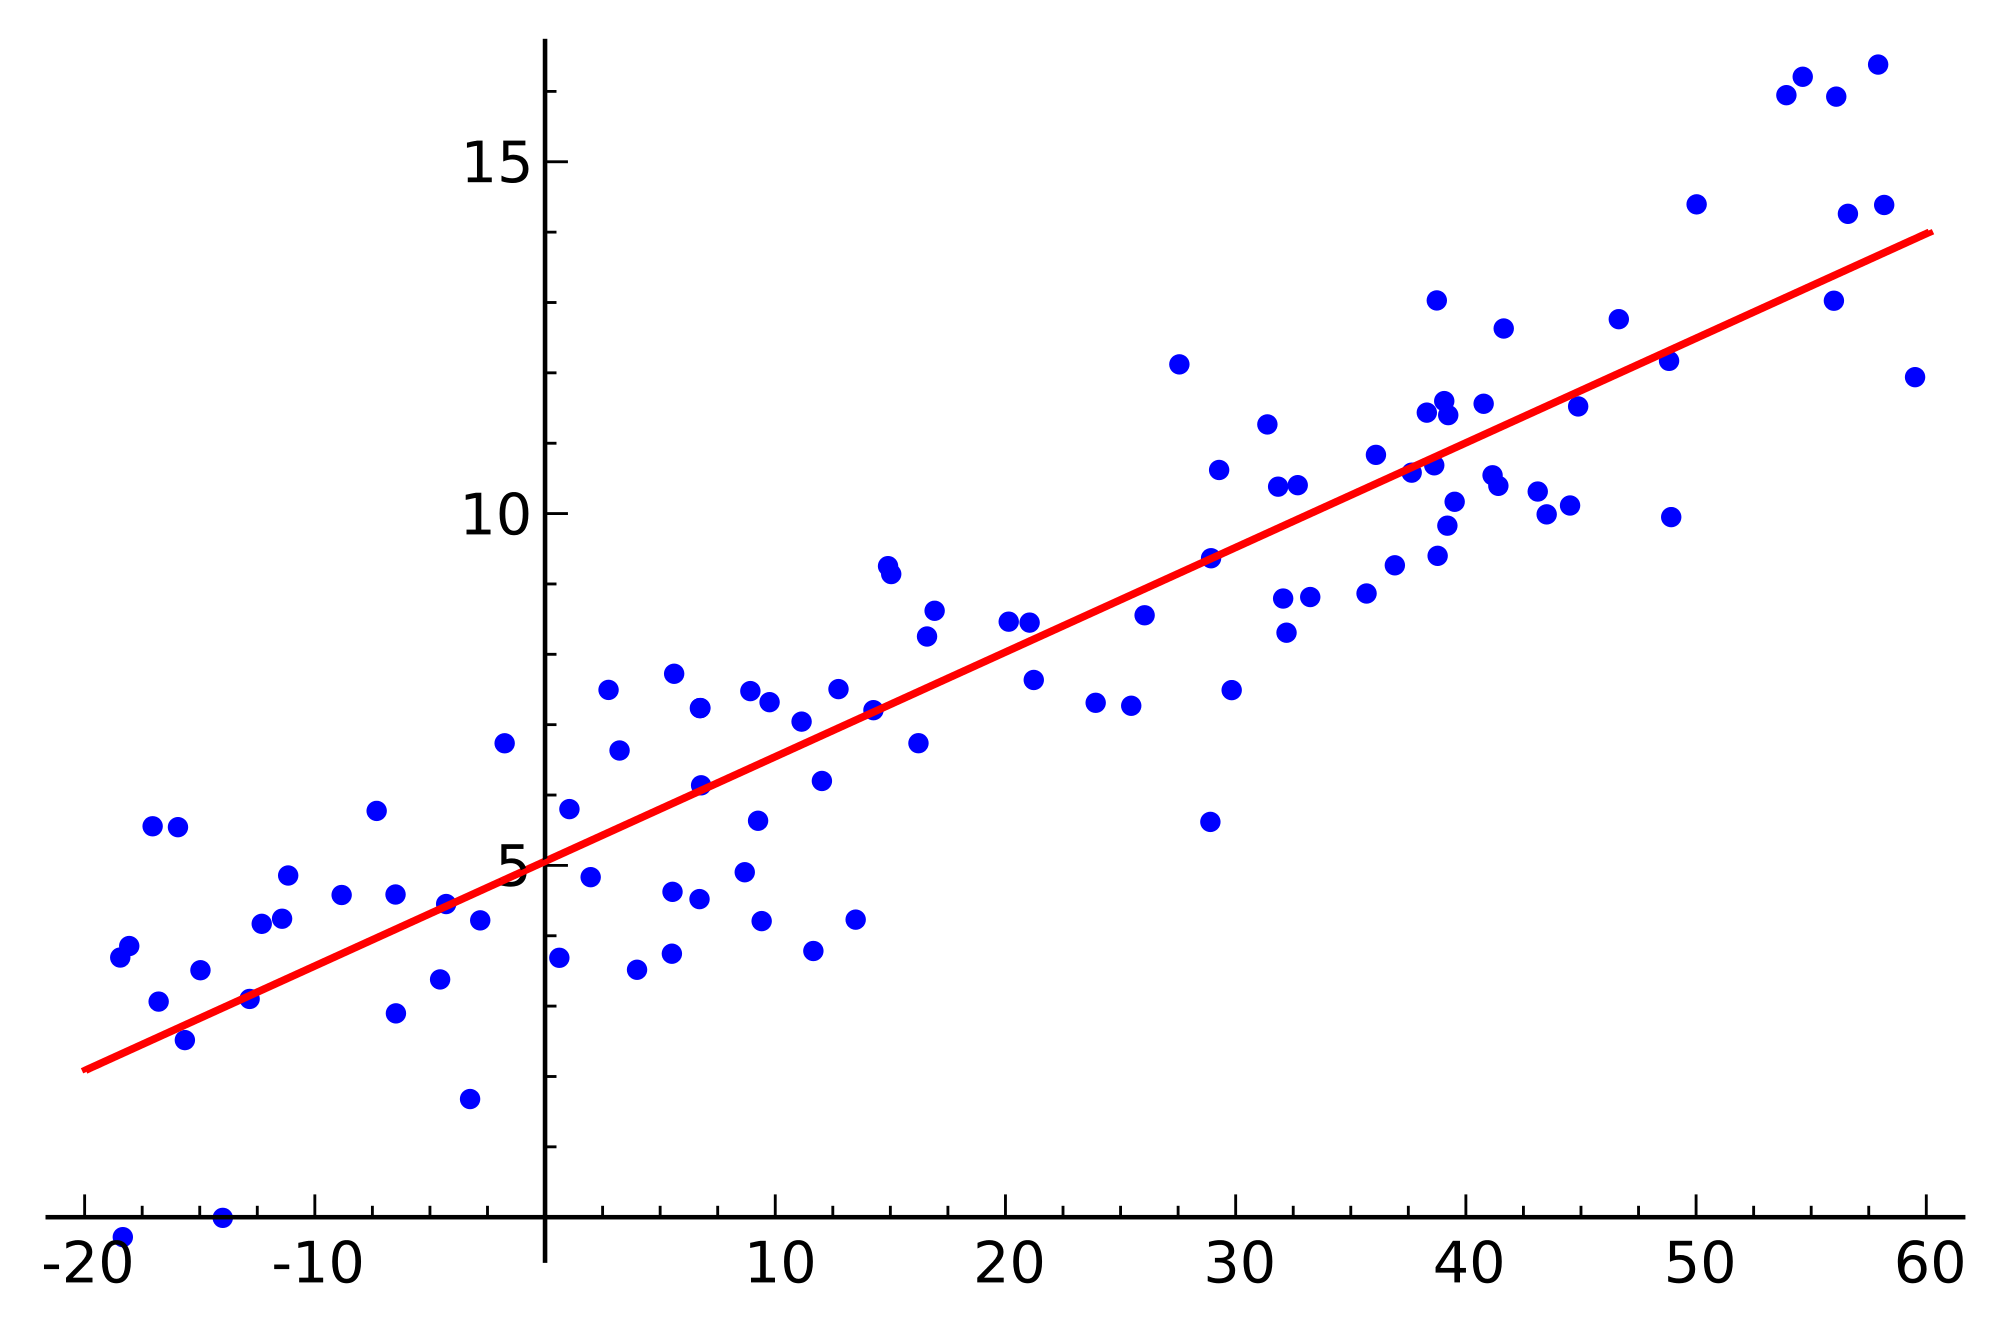
\includegraphics[width=0.8\textwidth]{images/Linear_regression.png}
	\caption{Gerade einer einfachen linearen Regression durch eine Punktwolke}
	\source{\cite{Linear_regression_2017-01-08}}
	\label{fig:recherche:dataminingtechniken:disziplinen:regression}
\end{figure}

\subsection{Cluster analysis}
\label{sec:recherche:dataminingtechniken:disziplinen:clusteranalysis}
Die Cluster analysis (Clusteranalyse) weist, ähnlich zur \nameref{sec:recherche:dataminingtechniken:disziplinen:classification}, den Instanzen eine Klasse zu. Jedoch sind diese zu beginn nicht bekannt, wodurch es sich um ein \gls{unsupervisedlearning} handelt.

In \cref{fig:recherche:dataminingtechniken:disziplinen:clusteranalysis} sind Punkte in einem Koordinatensystem eingetragen. Diese werden bei der Clusteranalyse in mehrere Gruppen unterteilt, welche die Klassen abbilden. Im Gegensatz zur \nameref{sec:recherche:dataminingtechniken:disziplinen:classification} haben diese jedoch keine weitere Bedeutung sondern geben nur an, dass sie ähnlich zu allen anderen Instanzen im selben Cluster sind. Je nach Verfahren ist es unterschiedlich, wie viele Klassen gebildet werden oder ob die Anzahl vorgegeben ist\footcite{data_mining_concepts_and_techniques}.
\begin{figure}[H]
	\RawFloats
	\centering
	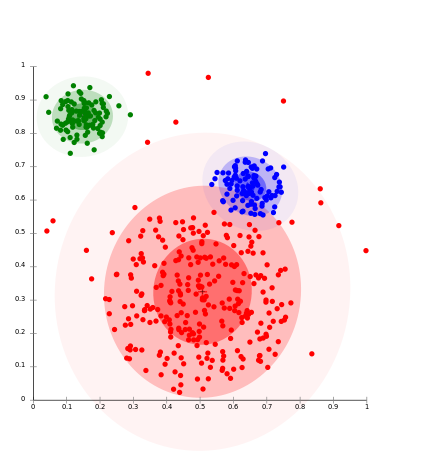
\includegraphics[width=0.8\textwidth]{images/clusteranalysis.png}
	\caption{Koordinatensystem für eine Cluster analysis}
	\source{\cite{Cluster_analysis_2017-01-08}}
	\label{fig:recherche:dataminingtechniken:disziplinen:clusteranalysis}
\end{figure}

Eingesetzt wird die Clusteranalyse zum Beispiel für die Erkennung von Kundengruppen oder zur  Zusammenfassung und Vergleich gleichartiger Produkten\footcite{einsatzgebiet_clusteranalyse}.


\subsection{Collaborative Filtering}
\label{sec:recherche:dataminingtechniken:disziplinen:collaborativefiltering}
Beim Collaborative Filtering werden Verhaltensmuster von Benutzern analysiert um daraus Empfehlungen für andere Kunden zu generieren. Am Beispiel einer Videotheke sind die einzelnen Instanzen die Filme, und die Empfehlungen die Bewertungen der Filme durch die Kunden. 

In der \cref{fig:recherche:dataminingtechniken:disziplinen:collaborativefiltering} sind in den Zeilen Filme (Instanzen) aufgeführt und in den Spalten die Kunden. Ein Feld stellt eine Bewertungen eines Kunden dar. "`+"' steht für eine positive und "`-"' für eine negative Bewertung. Leere Felder bedeutet dass der Kunde diesen Film nicht bewertet hat. Mittels kollaborativen Filtern kann nun vorhergesagt werden, ob ein Benutzer die gelb hinterlegte Instanz positiv oder negativ bewertet\footcite{collaborative_filtering}.
\begin{table}[H] 
	\caption{Beispiel von Collaborative Filtering einer Videotheke}
	\centering
	\rowcolors{1}{tablebodycolor}{tablerowcolor}
	\label{fig:recherche:dataminingtechniken:disziplinen:collaborativefiltering}
	
	\begin{tabular}{ | l | c | c | c | c |} 
		\hline 
		\rowcolor{tableheadcolor}
		\bfseries & 
		\bfseries Maria & 
		\bfseries Sandro & 
		\bfseries Urs & 
		\bfseries Heidi \\ \hline 
		\textbf{Pulp Fiction} & - & - &  & + \\ \hline 
		\textbf{The Matrix} & + & + & + & - \\ \hline 
		\textbf{American Hustle} & - & + &  & + \\ \hline 
		\textbf{12 Monkeys} & + & + & - & \cellcolor{yellow!75}? \\ \hline 
	\end{tabular} 
\end{table}

\section{Algorithmen}
\label{sec:recherche:algorithmen}
Hier werden drei Algorithmen aus den Problembeschreibungen im \cref{sec:recherche:dataminingtechniken:disziplinen} \nameref{sec:recherche:dataminingtechniken:disziplinen} beschrieben. Die Auswahl dieser Vorgehensweisen wird im Konzept erläutert (siehe \cref{sec:konzept:disziplin-und-algorithmen} \nameref{sec:konzept:disziplin-und-algorithmen}).

\subsection{Association rule learning: Apriori}
\label{sec:recherche:apriori}
Der Apriori Algorithmus ist der erste von zwei Schritten des \nameref{sec:recherche:dataminingtechniken:disziplinen:association} (\cref{sec:recherche:dataminingtechniken:disziplinen:association}), dessen Ziel es ist häufige Attribut-Kombinationen aufzufinden. 

Nachfolgend wird der Ablauf des Algorithmus erklärt.
Als Parameter verlangt dieser den Mindestsupport $minsup$ welcher definiert, wie oft eine Attributmenge $C$ in Instanzen $I$ in der Datenmenge $D$ vorkommen muss, damit diese als relevant betrachtet werden.
\begin{enumerate}
	\item Zähle die Vorkommen von allen Attributen und fasse das Resultat in $C_1$ (Kandidaten (candidates) 1-Attributmengen) zusammen.
	\item Entferne Elemente aus $C_1$ welche $minsup$ nicht erfüllen und speichere das Resultat in $L_1$ (frequente 1-Attributmengen).
	\item Setze $k=2$
	\item Solange $L_{k-1} \neq \emptyset$:
	\begin {enumerate}
	\item Generiere alle Möglichen Kombinationen für $C_k$ aus $L_{k-1}$ (apriori\_gen).
	\item Entferne Elemente aus $C_k$ welche $minsup$ nicht erfüllen und speichere das Resultat in $L_k$.
	\item Erhöhe $k$ um eins.
\end{enumerate}
\item Das Resultat sind alle Elemente in $L_k$.
\end{enumerate}

Als erstes (Schritte 1-2) werden alle einzelnen Attribute (1-Attributmenge) gezählt und diejenigen entfernt, welche $minsup$ nicht erfüllen.

Danach wird Iterativ die Attributmenge um ein Element erweitert und wiederum auf $minsup$ überprüft, bis keine Elemente mehr den Mindestsupport erreichen (Schritt 3).

Vereinfacht dargestellt ist der Punkt 3.a. Dieser Schritt heisst apriori\_gen und seine Aufgabe ist es, die häufigen Attriutmengen für die nächste Iteration zu generieren. Er nimmt die Liste mit den frequentierten Datensätzen der vorherigen Iteration ($L{k-1}$) und erweitert alle Mengen um ein Element. Er macht sich die Eigenschaft zunutze, dass wenn in $L_{k-1}$ ein Element $minsup$ nicht erfüllt, kann es dies auch nicht in $C_k$, wodurch $C_k$ verkürzt und der Algorithmus beschleunigt wird\footcite{data_mining_concepts_and_techniques}.

In der \cref{fig:recherche:vorgehensweise:apriorialgorithmus} wird der Ablauf am Beispiel eines Warenkorbes veranschaulicht.

\begin{figure}[H]
\RawFloats
\centering
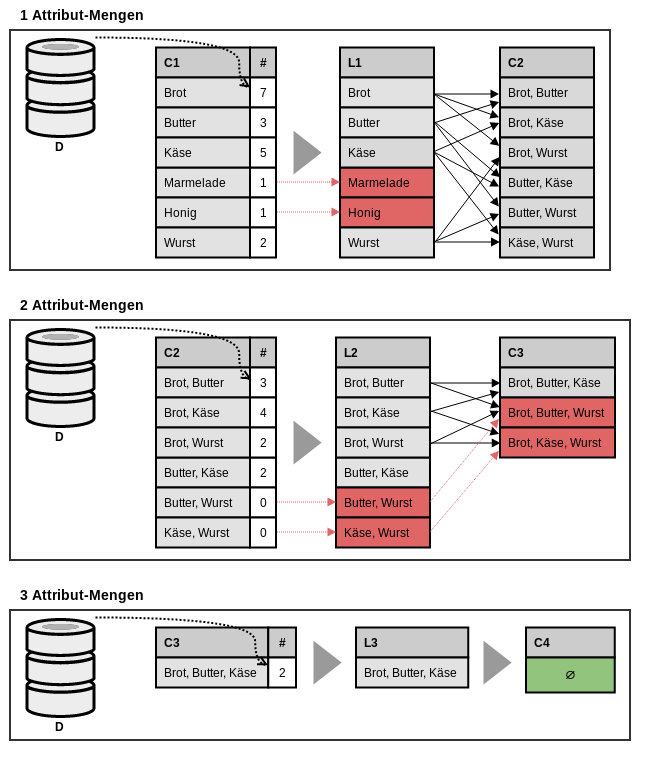
\includegraphics[width=0.8\textwidth]{images/Apriori-Algorithmus.png}
\caption{Visualisierung des Apriori Algorithmus}
\source{\cite{association_rule_learning_2017-01-05}}
\label{fig:recherche:vorgehensweise:apriorialgorithmus}
\end{figure}

$D$ wird benötigt um die Vorkommen zu zählen. Die roten Elemente in $L_k$ werden entfernt weil $minsup$ nicht erreicht wurde, welches im Beispiel den Wert 2 hat. Nach der Säuberung von $L_k$ erstellt der apriori\_gen die Kandidaten $C_k$ für den nächsten durchlauf (join). Anschliessend werden in $C_k$ diejenigen Elemente entfernt, welche in $L_{k-1}$ als nicht häufig erkannt wurde (prune). Zum Beispiel kann in $C_3$ das Element {Brot, Butter, Wurst} entfernt werden, da in $L_2$ {Butter, Wurst} den Wert $minsup$ unterschreitet.

Der Algorithmus wird gestoppt, wenn es keine häufigen Kandidaten mehr gibt, was in $C_4$ der Fall ist.

Der Algorithmus kann somit in drei Schritte aufgeteilt werden.
\begin{enumerate}
\item Häufigkeitszählung
\item Generierung der x+1-Attributmenge (Apriori-gen Funktion, join step)
\item Entfernung der Elemente welche den $minsup$ nicht erfüllen (Apriori-gen Funktion, prune step)
\end{enumerate}

Die nachfolgende Apriori-Methode führt die Häufigkeitszählung durch.
Gegeben ist die gesamte Datenmenge $D$, welche für die Häufigkeitszählung verwendet wird, sowie der minimum Support $minsup$ welche die Attribute zu erfüllen haben.
\begin{lstlisting}[language=pseudocode]
procedure apriori($D$: Datenmenge; $minsup$: Minimum support) {
	$L_1 \gets$ find_frequent_1%-%itemsets($D$)
	$k \gets 2$
	while $L_{k-1} \neq \emptyset$ {
		$C_k \gets$ apriori_gen($L_{k-1}$)
		foreach transaction $I \in D$ {
			$C_I \gets \{ c | c \in C_k \wedge c \subseteq I \}$
			foreach candidate $c \in C_I$ {
				count[$c$] $\gets$ count[$c$] + 1
			}
		}
		$L_k \gets \{c | c \in C_k \wedge$ count[$c$] $\ge minsup \}$
		$k \gets k + 1$
	}
	return $\bigcup\limits_{k} L_{k}$
}
\end{lstlisting}
Im ersten Schritt wird die 1-Attributmenge mit häufigen Elementen definiert. In den Zeilen 3 bis 14 wird für $k > 2$ die Items gesammelt, welche öfters vorkommen als der $minsup$. Dazu wird mittels der apriori\_gen Funktion die \textit{Candidates} $C_k$ generiert (Zeile 5).
Anschliessend werden die vorkommen von allen Elementen in $D$ gezählt, wie oft sie in $C_k$ vorkommen (Zeilen 6-12).


\begin{lstlisting}[language=pseudocode]
procedure apriori_gen($L_{k-1}$:frequent %(k-1)-%itemsets) {
	$C_k \gets \emptyset$
	foreach itemset $l_1 \in L_{k-1}$ {
		foreach itemset $l_2 \in L_{k-1}$ {
			$c \gets \{l_1 \cup \{i\} | i \in l_2 \wedge l_1 \cup \{i\} \notin C_k \}$
			$c_{pruned} \gets c - \{ c' | c' \in c \wedge i \subset c \wedge |i| = k-1 \wedge i \notin L_{k-1} \}$
			$C_k \gets C_k \cup c_{pruned}$
		}
	}
	return $C_k$
}
\end{lstlisting}
In der apriori\_gen Funktion werden k-Attributmengen generiert, indem eine (k-1)-Attributmenge erweitert wird. Dazu gibt es zwei Schleifen welche durchlaufen werden. Auf Zeile 5 wird $l_1$ um Elemente von $l_2$ erweitert. Zudem wird sichergestellt, dass gleiche Mengen nicht mehrfach in $C_k$ hinzugefügt werden können.

Auf Zeile 6 werden die k-Attributmengen gesäubert (prune), indem die neuen Kandidaten $c$ überprüft werden, ob eine Submenge $i$ eines Kandidaten $c'$ nicht in $L_{k-1}$ vorhanden ist. Wenn dies der Fall ist erfüllt $i$ den $minsup$ womit $c'$ den mindest support auch nicht erfüllen kann. Somit kann $c'$ aus $c$ entfernt werden.

% Longer version of apriori_gen
%$c \gets \{l_1 \cup \{i\} | i \in l_2 \wedge l_1 \cup \{i\} \in C_k \}$
%$c_{pruned} \gets \{ i | i \in c \wedge \forall j(j \subset i \wedge |j| = k-1 \wedge j \in L_{k-1}) \}$
%$C_k \gets C_k \cup c_{pruned}$
%
% Looped version of apriori_gen
%	$C_k \gets \emptyset$
%	foreach itemset $l_1 \in L_{k-1}$ {
%		foreach itemset $l_2 \in L_{k-1}$ {
%			if (($l_1$[1] = $l_2$[1]) $\wedge$ ($l_1$[2] = $l_2$[2]) $\wedge$ ... $\wedge$ ($l_1$[$k$-2] = $l_2$[$k$-2]) $\wedge$ ($l_1$[$k$-1] $<$ $l_2$[$k$-1])) {
%				$c \gets l_1 \cup l_2$
%				if not has_infrequent_subset($c, L_{k-1}$) {
%					delete $c$
%				} else {
%					$C_k \gets C_k \cup c$
%					add $C_k \cup c$ 
%				}
%			}
%		}
%	}
%	return $C_k$
%
%
%\begin{lstlisting}
%procedure has_infrequent_subset($c$: candidate k-itemset; $L_{k-1}$: frequent (k-1)-itemsets) {
%	foreach (k-1)-subset $s of c$ {
%		if $s \notin L_{k-1}$ {
%			return TRUE
%		}
%	}
%	return FALSE
%}
%\end{lstlisting}


\subsection{Cluster analysis: k-prototype}
\label{sec:recherche:algorithmen:k-prototypes}
Die k-prototypes Vorgehensweise gehört zu der Gruppe der partitionierenden Clustering Algorithmen. Er ist eine Kombination des Lloyd- und des \gls{pam}- Algorithmus. Er verwendet eine angepasste Version der quadratischen euklidischen Distanz (siehe \cref{sec:konzept:algorithmenauswahl:clustering} \nameref{sec:konzept:algorithmenauswahl:clustering}), wie sie Lloyd verwendet und benutzt für die Zentren der Clusters Medoiden, wie dies der \gls{pam} Algorithmus macht\footcite{data_mining_concepts_and_techniques}\footcite{clustering_numeric_and_categorical_values}. Im k-prototype heissen die Zentren nicht Medoiden, sondern "`Prototyp"', woher auch der Name kommt.

Der Ablauf von k-prototypes besteht aus fünf Schritten\footcite{clustering_numeric_and_categorical_values}:
\begin{enumerate}
	\item Initiale Prototypen-Auswahl $\{o_1,\ldots,o_k\}$. Diese bilden die ersten Cluster.
	\item Alloziere jede Instanz zu ihrem nächsten Prototypen.
	\item Wähle zufällig einen Prototypen $o_{random}$ als Ersatz für den aktuellen Prototypen $o_j$ einses Clusters.
	\item Berechne die Kosten $E_{random}$ welche die durch eine Änderung von $o_j$ durch $o_{random}$ entstehen.
	\item \textbf{if} $E_j > E_{random}$ \textbf{then} Ersetze $o_j$ durch $o_{random}$ und wiederhole 2.-5. bis keine Änderungen an den Clustern mehr vorgenommen werden.
\end{enumerate}

Der neue Prototypen in Schritt 3. wird zufällig ausgewählt. Dadurch findet der Algorithmus ein lokales Optimum, jedoch nicht zwingend das beste Resultat\footcite{data_mining_concepts_and_techniques}.
Die Funktion für die Kostenberechnung im Schritt 4 wird im \cref{sec:konzept:algorithmenauswahl:clustering:distanzmessung} vorgestellt.

Die Laufzeit des Algorithmus ist $\mathcal{O}((t+1)kn)$, wobei $n$ die Anzahl Instanzen, $k$ die Anzahl Cluster und $t$ die Anzahl der Iterationen darstellt. Üblicherweise ist $k \ll n$ und $t < 100$, wodurch der Algorithmus sehr effizient ist und auch auf grossen Datenbeständen angewendet werden kann\footcite{clustering_numeric_and_categorical_values}.

\subsection{Cluster analysis: DBSCAN}
\label{sec:recherche:algorithmen:dbscan}
\gls{dbscan} gehört zu der Gruppe der Density-based Clustering Algorithmen. 
Vorgegeben werden muss der Radius $\epsilon$ und die minimum Anzahl an Instanzen $minpts$. Ein Cluster wird gebildet wenn um einen Punkt im Radius $\epsilon$ mindestens $minpts$ andere Instanzen liegen. Mit diesen Informationen kann der Algorithmus in einer Laufzeit von $\mathcal{O}(n\,log\,n)$ ein Clustering durchführen.

Der Algorithmus führt mehrere Begriffe ein\footcite{data_mining_concepts_and_techniques}:
\begin{itemize}
	\item \textit{neighborhood density}: Wie viele Instanzen befinden sich im Radius von $\epsilon$ um einen Punkt $p$. 
	\begin{equation}
	\mathit{ND}_{\epsilon}(p) = \{q | q \in D \wedge d(p,q) < \epsilon\}
	\end{equation}
	\item \textit{core object}: Instanz welche mindestens $minpts$ in der Nachbarschaft haben.
	\begin{equation}
	|\mathit{ND}_{\epsilon}(p)| \geq minpts
	\end{equation}
	\item \textit{noise}: Instanz für welche weniger als $minpts$ in der Nachbarschaft haben.
	\begin{equation}
	|\mathit{ND}_{\epsilon}(p)| < minpts
	\end{equation}
	\item \textit{directly density-reachable}: Alle Instanzen innerhalb des Radius $\epsilon$ um einen Punkt $q$, wenn $q$ ein \textit{core object} ist.
	\item \textit{density-reachable}: Punkt $p$ ist \textit{density-reachable} von $q$, wenn es Punkte $l_1,...,l_n$ gibt, so dass $l_1=q, l_n=p$ und $l_i+1$ \textit{directly density-reachable} von $l_i$ aus ist, für $1 \leq i \leq n$.
	\item \textit{density-connected}: Wenn es zwei \textit{core objects} $p_1,p_2$ und einen Punkt $q$ gibt, so dass $p_1$ und $p_2$ \textit{density-reachable} von $q$ aus sind.
\end{itemize}

Die Unterscheidung zwischen \textit{density-reachable} und \textit{density-connected} ist notwendig, da ersteres Kriterium asymmetrisch und letzteres symmetrisch ist. Veranschaulicht wird dies in \cref{fig:recherche:clusteranalysis:DBSCAN}.

\begin{figure}[H]
	\RawFloats
	\centering
	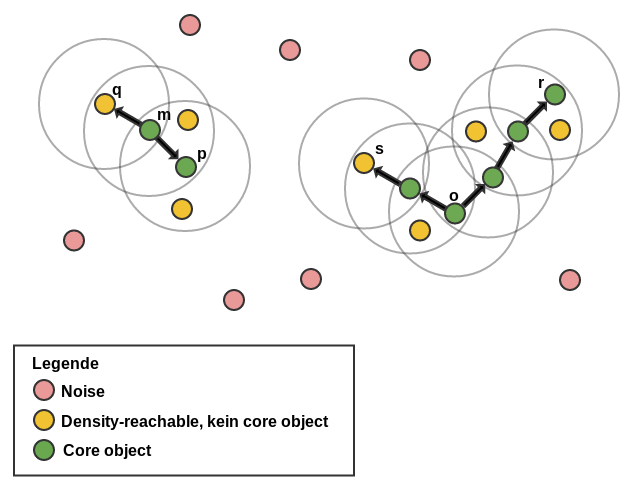
\includegraphics[width=0.8\textwidth]{images/density-reachable-vs-connected.png}
	\caption{density-reachable vs density-connected}
	\source{\cite{data_mining_concepts_and_techniques}}
	\label{fig:recherche:clusteranalysis:DBSCAN}
\end{figure}

Punkte m,p,o und r sind \textit{core objects} da sich in den Radien $\epsilon$ mindestens 3 andere Instanzen ($minpts = 3$) befinden. Da m und p beides \textit{core objects} sind, sind beide Punkte untereinander \textit{density-reachable}. q ist \textit{density reachable} von m und von p aus, jedoch nicht umgekehrt, da q kein \textit{core object} ist. 

Auf der rechten Seite sind r und s \textit{density-rechable} von Punkt o, weshalb r,s und o untereinander \textit{density-connected} sind.

Clusters werden mit den Punkten gebildet, welche untereinander \textit{density-connected} sind. 
Der Algorithmus geht folgendermassen vor:

%\begin{enumerate}
%\item Markiere alle Punkte in $D$ als ''unvisited''.
%\item \textbf{foreach} $p$ \textbf{in} $\{d | d \in D \wedge d $ ist %''unvisited''$\}$
%\item \hspace{0.5cm}Markiere $p$ als ''visited''.
%\item \hspace{0.5cm}\textbf{if}  $|\mathit{ND}_{\epsilon}(p)| \geq minpts$ %\textbf{then} 
%\item \hspace{1cm} Erstelle einen Cluster für $p$.
%%\item \hspace{1cm} Füge alle Punkte aus $\mathit{ND}_{\epsilon}(p)$ in $N$ ein. %$N = \mathit{ND}_{\epsilon}(p)$
%\item \hspace{1cm} \textbf{foreach} $q$ \textbf{in} $N$
%\item \hspace{1.5cm} \textbf{if} $q$ ist ''unvisited'' \textbf{then}
%\item \hspace{2cm} Markiere $q$ als ''visited''.
%\item \hspace{2cm} Füge alle ''unvisited'' Instanzen aus %$\mathit{ND}_{\epsilon}(q)$ in $N$ ein.
%\end{enumerate}

\begin{lstlisting}
unvisited $\gets D$
inCluster $= \emptyset$
foreach itemset $p \gets$ unvisited {
	unvisited $\gets D - \{p\}$
	if $|\mathit{ND}_{\epsilon}(p)| \geq minpts$ {
		clusters[$p$] $\gets \{p\}$
		inCluster = inCluster $\cup p$
		candidates = $ND_{\epsilon}(p)$
		foreach $q \in $ candidates {
			// if q is unvisited.
			if $q \: \cap$ unvisited $\neq \varnothing$ {
				unvisited $\gets D - \{p\}$
				clusters[$p$] $\gets$ clusters[$p$] $ \cap$ $\{q\}$
				candidates $\gets$ candidates $\cup \: ND_{\epsilon}(q)$
			}
			// if q is not in a cluster yet.
			if $q \: \cap$ inCluster $= \varnothing$ {
				clusters[$p$] = cluster[$p$] $\cup q$
			}
		}
	}
}
\end{lstlisting}
Zu Beginn werden alle Punkte als "`unvisited"' makriert. Anschliessend wird ein zufälliger Punkt $p$ gewählt welcher als "`visited"' markiert wird. Auf Zeile 4 wird überprüft ob die \textit{neighborhood density} von $p$ den mindestwert $minpts$ erfüllt. Wenn ja wird für diesen Punkt ein Cluster erstellt und all seine Nachbaren in "`candidates"' gespeichert. Schlussendlich überprüfen ob die "`candidates"' noch "`unvisited"' sind (Zeile 8). Wenn ja wird der Kandidat $q$ als "`visited"' markiert (Zeile 9), in den Cluster $p$ eingefügt (Zeile 10)und all seine Nachbaren der Liste "`candidates"' angehängt (Zeile 11).

Abgebrochen wird wenn alle Punkte als "`visited"' markiert sind.

\section{Wissenschaftliche Arbeiten}
Es wurde im Netz nach bestehenden wissenschaftlichen Arbeiten gesucht, die sich mit der Thematik dieser Arbeit bereits auseinandergesetzt hat. Der Apriori Algorithmus wird üblicherweise in Verbindung mit dem Association rule learning verwendet und nur selten für die reine Häufigkeitsanalyse eingesetzt. Deshalb wurden nur wenige Berichte gefunden welche sich rein auf den Apriori beziehen. 
Zum Beispiel wird im Bericht "`An Apriori-based Algorithm for Mining Frequent Substructures from Graph Data"'\footcite{agm} der Apriori Algorithmus auf einer graphischen Repräsentation von chemischen Verbindungen ausgeführt. Eingesetzt wird er zur Auffindung von häufig auftretenden induzierten Subgraphen. Gemäss dem Fazit ist der Algorithmus gut geeignet um effizient Häufigkeiten aufzudecken. Obwohl das Einsatzgebiet und die Datenstrukturen des Berichtes sehr unterschiedlich sind zu dieser Arbeit sollte der Apriori Algorithmus trotzdem anwendbar sein und effiziente zu einem Resultat führen.

\section{Programmevaluation}
\label{sec:recherche:programmevaluation}
Auf dem Markt gibt es diverse Data Mining Programme von welchen hier einige vorgestellt werden.

Zwingend notwendig ist es, dass das Programm gratis ist, sowie unter den Betriebsystemen Windows sowie Linux lauffähig ist. 

%http://thenewstack.io/six-of-the-best-open-source-data-mining-tools/

\subsection{RapidMiner Studio}
RapidMiner, früher YALE (Yet Another Learning Environment) wurde von der Technischen Universität Dortmund entwickelt und bietet eine kostenlose Version an, welche auf 10'000 Datensätze und einen logischen Prozessor beschränkt ist. Es gibt jedoch für Studenten eine Version mit welcher beliebig Grosse Daten bearbeitet werden können. Die Applikation ist in Java geschrieben und somit auf allen gängigen Betriebssystemen lauffähig\footcite{RapidMiner_Studio_2017-01-14}.

RapidMiner Studio bietet für eine grosse Anzahl an Algorithmen fertige Bausteine an, welche verwendet werden können. Alle unter \cref{sec:recherche:dataminingtechniken:disziplinen} aufgeführten Methoden sind in der Applikation als Operatoren implementiert und können durch einige klicks verwendet werden. Eine Auflistung aller Operatoren ist in der RapidMiner Dokumentation aufgeführt: \url{http://docs.rapidminer.com/studio/operators/}

\subsection{Weka}
\gls{weka} ist ein in Java entwickeltes Programm der University of Waikato, New Zealand. Veröffentlicht wurde die Software unter der \gls{acr:gnugpl} und ist somit frei verfüg- und modifizierbar\footcite{Weka_2017-01-14}.

WEKA beherscht Classification, Clustering, lineare Regression und Associating Algorithmen und deckt somit alle  im \cref{sec:recherche:dataminingtechniken:disziplinen} aufgeführten Disziplinen ab\footcite{Weka_Doc_2017-01-14}\footcite{Weka_Regression_2017-01-14}.

